% Options for packages loaded elsewhere
\PassOptionsToPackage{unicode}{hyperref}
\PassOptionsToPackage{hyphens}{url}
\PassOptionsToPackage{dvipsnames,svgnames,x11names}{xcolor}
%
\documentclass[
  12pt,
]{article}
\usepackage{amsmath,amssymb}
\usepackage{lmodern}
\usepackage{iftex}
\ifPDFTeX
  \usepackage[T1]{fontenc}
  \usepackage[utf8]{inputenc}
  \usepackage{textcomp} % provide euro and other symbols
\else % if luatex or xetex
  \usepackage{unicode-math}
  \defaultfontfeatures{Scale=MatchLowercase}
  \defaultfontfeatures[\rmfamily]{Ligatures=TeX,Scale=1}
\fi
% Use upquote if available, for straight quotes in verbatim environments
\IfFileExists{upquote.sty}{\usepackage{upquote}}{}
\IfFileExists{microtype.sty}{% use microtype if available
  \usepackage[]{microtype}
  \UseMicrotypeSet[protrusion]{basicmath} % disable protrusion for tt fonts
}{}
\makeatletter
\@ifundefined{KOMAClassName}{% if non-KOMA class
  \IfFileExists{parskip.sty}{%
    \usepackage{parskip}
  }{% else
    \setlength{\parindent}{0pt}
    \setlength{\parskip}{6pt plus 2pt minus 1pt}}
}{% if KOMA class
  \KOMAoptions{parskip=half}}
\makeatother
\usepackage{xcolor}
\IfFileExists{xurl.sty}{\usepackage{xurl}}{} % add URL line breaks if available
\IfFileExists{bookmark.sty}{\usepackage{bookmark}}{\usepackage{hyperref}}
\hypersetup{
  colorlinks=true,
  linkcolor={RoyalBlue},
  filecolor={Maroon},
  citecolor={Blue},
  urlcolor={RoyalBlue},
  pdfcreator={LaTeX via pandoc}}
\urlstyle{same} % disable monospaced font for URLs
\usepackage[margin=1in]{geometry}
\usepackage{graphicx}
\makeatletter
\def\maxwidth{\ifdim\Gin@nat@width>\linewidth\linewidth\else\Gin@nat@width\fi}
\def\maxheight{\ifdim\Gin@nat@height>\textheight\textheight\else\Gin@nat@height\fi}
\makeatother
% Scale images if necessary, so that they will not overflow the page
% margins by default, and it is still possible to overwrite the defaults
% using explicit options in \includegraphics[width, height, ...]{}
\setkeys{Gin}{width=\maxwidth,height=\maxheight,keepaspectratio}
% Set default figure placement to htbp
\makeatletter
\def\fps@figure{htbp}
\makeatother
\setlength{\emergencystretch}{3em} % prevent overfull lines
\providecommand{\tightlist}{%
  \setlength{\itemsep}{0pt}\setlength{\parskip}{0pt}}
\setcounter{secnumdepth}{-\maxdimen} % remove section numbering
\newlength{\cslhangindent}
\setlength{\cslhangindent}{1.5em}
\newlength{\csllabelwidth}
\setlength{\csllabelwidth}{3em}
\newlength{\cslentryspacingunit} % times entry-spacing
\setlength{\cslentryspacingunit}{\parskip}
\newenvironment{CSLReferences}[2] % #1 hanging-ident, #2 entry spacing
 {% don't indent paragraphs
  \setlength{\parindent}{0pt}
  % turn on hanging indent if param 1 is 1
  \ifodd #1
  \let\oldpar\par
  \def\par{\hangindent=\cslhangindent\oldpar}
  \fi
  % set entry spacing
  \setlength{\parskip}{#2\cslentryspacingunit}
 }%
 {}
\usepackage{calc}
\newcommand{\CSLBlock}[1]{#1\hfill\break}
\newcommand{\CSLLeftMargin}[1]{\parbox[t]{\csllabelwidth}{#1}}
\newcommand{\CSLRightInline}[1]{\parbox[t]{\linewidth - \csllabelwidth}{#1}\break}
\newcommand{\CSLIndent}[1]{\hspace{\cslhangindent}#1}
\usepackage{setspace}\doublespacing
\usepackage[left]{lineno}
\ifLuaTeX
  \usepackage{selnolig}  % disable illegal ligatures
\fi

\author{}
\date{\vspace{-2.5em}}

\begin{document}

\pagenumbering{arabic}

\linenumbers

Title: Ten simple rules for working with high-resolution remote sensing
data

Adam L. Mahood\textsuperscript{1,2,\texttt{*}}, Maxwell B.
Joseph\textsuperscript{1}, Anna I. Spiers\textsuperscript{1,3}, Michael
J. Koontz\textsuperscript{1}, Nayani Ilangakoon\textsuperscript{1},
Kylen Solvik\textsuperscript{1,2}, Nathan Quarderer\textsuperscript{1},
Joe McGlinchy\textsuperscript{1}, Victoria M.
Scholl\textsuperscript{1,2}, Lise St.~Denis\textsuperscript{1}, Chelsea
Nagy\textsuperscript{1,2}, Anna Braswell\textsuperscript{4,5}, Matthew
W. Rossi\textsuperscript{1}, Lauren Herwehe\textsuperscript{1,2}, Leah
Wasser\textsuperscript{1,2}, Megan E. Cattau\textsuperscript{6},
Virginia Iglesias\textsuperscript{1}, Fangfang Yao\textsuperscript{2},
Stefan Leyk\textsuperscript{1,2,7}, Jennifer K.
Balch\textsuperscript{1,2},

\textsuperscript{1} Department of Geography, University of Colorado
Boulder, Boulder, CO, USA

\textsuperscript{2} Earth Lab, University of Colorado, Boulder, CO, USA

\textsuperscript{3} Department of Ecology and Evolutionary Biology,
University of Colorado Boulder, Boulder, CO, USA

\textsuperscript{4} School of Forest, Fisheries, and Geomatic Sciences,
Institute of Food and Agricultural Sciences, University of Florida,
Gainesville, FL, USA

\textsuperscript{5} Florida Sea Grant, Institute of Food and
Agricultural Sciences, University of Florida, Gainesville, USA

\textsuperscript{6} Department of Human-Environment Systems, Boise State
University, Boise, ID, USA

\textsuperscript{7} Institute of Behavioral Science, University of
Colorado Boulder, Boulder, CO, USA

\texttt{*} Corresponding author:
\href{mailto:admahood@gmail.com}{\nolinkurl{admahood@gmail.com}}

\hypertarget{abstract}{%
\section{Abstract}\label{abstract}}

Researchers in Earth and environmental science can extract incredible
value from high-resolution (sub-meter, sub-hourly or hyper-spectral)
remote sensing data, but these data can be difficult to use. Correct,
appropriate and competent use of such data requires skills from remote
sensing and the data sciences that are rarely taught together. In
practice, many researchers teach themselves how to use high-resolution
remote sensing data with ad hoc trial and error processes, often
resulting in wasted effort and resources. In order to implement a
consistent strategy, we outline ten ``rules'' with examples from Earth
and environmental science to help academic researchers and professionals
in industry work more effectively and competently with high-resolution
data.

\hypertarget{introduction}{%
\section{Introduction}\label{introduction}}

The data revolution brings a deluge of Earth observations from numerous
and diverse sensors. Many of these data are collected remotely: from
space, the air, or underwater, and are of increasingly high-resolution,
providing detailed spatial, temporal, radiometric, and/or spectral
information (Figure 1). Earth and environmental scientists as well as
professionals with analytical or computational backgrounds increasingly
use high-resolution remote sensing data, but learning how to do this
correctly and effectively can be difficult. In this article, we outline
ten simple rules to help Earth and environmental researchers make
informed decisions about the use and benefits of high-resolution remote
sensing data.

Current understanding of high-resolution may include sub-meter,
sub-hourly or hyper-spectral, but this is constantly changing, and what
is considered high-resolution has to be considered in the context of the
spatial and temporal coverage. We may even be reaching the useful limits
of resolution with some products, but at limited coverage, or
high-resolution in one aspect but low in others (Figure 2). For example,
the Geostationary Operational Environmental Satellites (GOES,
\protect\hyperlink{ref-schmidt_goes_2003}{Schmidt and Prins 2003}) have
sub-hourly resolution for most of the western hemisphere, but low (1.5
km) spatial resolution. Future advances may center around increasing the
resolution of all facets of a single product. For example, Landsat and
Sentinel are considered moderate resolution in all facets, but with
global coverage, and have been progressing towards higher resolution in
all facets since the first Landsat satellite was launched in 1972.
Landsat 8 has higher spatial and spectral resolution than previous
Landsat products (\protect\hyperlink{ref-roy2014landsat}{Roy et al.
2014}). Now, with the launch of Landsat 9
(\protect\hyperlink{ref-masek2020landsat}{Masek et al. 2020}), the
temporal resolution is doubled. Furthermore, the Landsat products have
since been harmonized with Sentinel 2 for a unified product with even
higher temporal resolution
(\protect\hyperlink{ref-claverie2018harmonized}{Claverie et al. 2018}).
See Table 1 for more information on the data products we refer to
throughout this article.

The use of high-resolution data allow us to answer persistent science
questions in different ways, and to ask new questions altogether. For
instance, the Shuttle Radar Topography Mission (SRTM) generated a
near-global digital elevation model (DEM) at 30m resolution at the turn
of the century (\protect\hyperlink{ref-farr2000shuttle}{Farr and Kobrick
2000}), and this enabled new insights into hydrography
(\protect\hyperlink{ref-lehner2008new}{Lehner, Verdin, and Jarvis
2008}), cryology
(\protect\hyperlink{ref-surazakov2006estimating}{Surazakov and Aizen
2006}), vegetation remote sensing
(\protect\hyperlink{ref-simard2006mapping}{Simard et al. 2006}), climate
change-induced coastal flood risk
(\protect\hyperlink{ref-mcgranahan2007rising}{McGranahan, Balk, and
Anderson 2007}), limnology (\protect\hyperlink{ref-nasa2013}{NASA 2013})
and more. But, what defines ``high-resolution'' changes over time, and a
30m DEM is considered moderate resolution today, relative to sub-meter
topography data that are increasingly available and yield finer detail
and thus new insights
(\protect\hyperlink{ref-kruse2015validation}{Kruse, Baugh, and Perry
2015}; \protect\hyperlink{ref-thatcher20203d}{Thatcher, Lukas, and
Stoker 2020}; \protect\hyperlink{ref-wang2021flood}{C. Wang et al.
2021}). For instance, analysis based on a novel integration of SRTM with
higher resolution elevation data derived from Light Detection and
Ranging (lidar) measurements tripled the estimate of the number of
people at risk worldwide from coastal flooding in the next century
(\protect\hyperlink{ref-kulp2019new}{Kulp and Strauss 2019}). High
temporal resolution has also led to recent advances. In another example,
Balch \emph{et al} (\protect\hyperlink{ref-balch_warming_2022}{2022})
used sub-hourly active fire detections across the western hemisphere to
advance our understanding of how climate change is impacting the diurnal
cycle of fire activity at a global scale.

Even though high-resolution data are valuable, they are not always easy
to use and can be of limited benefit in some cases. Effective and
informed use of high-resolution data requires remote sensing and data
science skills and theoretical knowledge
(\protect\hyperlink{ref-hampton2017skills}{Hampton et al. 2017}).
High-resolution data can be voluminous, complex, and noisy, requiring
systematic data and workflow management, data processing skills, and
in-depth uncertainty assessments. Further, high-resolution remote
sensing data are often integrated with other sources of information
(e.g., ground truth data or other environmental data), which brings
additional challenges associated with data harmonization,
reconciliation, and uncertainty propagation
(\protect\hyperlink{ref-zipkin2021addressing}{Zipkin et al. 2021}). In
practice, learning how to use high-resolution data is often an ad-hoc
trial and error process. The resulting bespoke approaches that
researchers develop can be inconsistent, inefficient, and challenging to
implement, reproduce, or extend.

Here we outline a set of ``rules'' to provide a foundation that
researchers can build upon to work effectively with high-resolution
data. We focus on examples in Earth and environmental science, but the
ideas apply to other disciplines.

\hypertarget{know-the-question}{%
\section{1. Know the question}\label{know-the-question}}

High-resolution data can enable refined, dynamic assessments of
environmental patterns and processes. It is thus important to prioritize
the formulation of the science question, understand its implications and
develop testable hypotheses (\protect\hyperlink{ref-betts2021}{Betts et
al. 2021}). An unambiguous question will guide the project and point to
a clear end , i.e., at what point has the question been answered, or has
the realization been reached that it cannot be answered as anticipated.
A clear question can also help with understanding data requirements
including spatial, temporal, radiometric, and spectral resolutions and
geographic extents (see Understand the data).

For example, a question about local plant population dynamics may need
high-resolution data to identify individual plants in a small region
(\protect\hyperlink{ref-koontz2021cross}{Koontz et al. 2021}). In
contrast, a question about vegetation and large-scale wildebeest
migration may require vegetation index data at a coarse spatial
resolution over a large geographic area
(\protect\hyperlink{ref-musiega2006framework}{Musiega, Sanga-Ngoie, and
Fukuyama 2006}). Finally, even high-resolution data may be sampled from
a large number of available data sources. If a science question requires
inference about this larger set of data sources, it is important to
understand whether the available sample of data permits inference, as
spatial bias in data availability can lead to unrepresentative samples,
complicating large-scale statistical inference
(\protect\hyperlink{ref-metcalfe2018patchy}{Metcalfe et al. 2018}).

To help organize your project and guide the data collection process,
clearly state a compelling science question
(\protect\hyperlink{ref-alon2009}{Alon 2009}). Know the scope and key
attributes of what is being analyzed, including scale, resolution, and
level of organization (e.g., individual, community, ecosystems,
landscape), to choose the most appropriate data. Consider how
representative/aligned or mismatched a sample is between the phenomenon
scale, the scale at which the feature or process of interest can be
measured, and the analytical scale, the scale that will be used as
dictated by the data resolution. Use domain expertise on your research
team to identify potential challenges at the interface of the question
and available data.

Identify the frontiers of research in the field and state a question. A
well-posed question points to data requirements and a clear end point.

\hypertarget{understand-the-data}{%
\section{2. Understand the data}\label{understand-the-data}}

In addition to defining the science question, it is important to know
the data. This includes knowing whether the available data are fit for
the intended use, given underlying assumptions, biases, strengths and
limitations. The concept of fitness for the use of a given data product
is useful for assessing the data quality
(\protect\hyperlink{ref-tayi1998examining}{Tayi and Ballou 1998})and its
appropriateness for the intended purpose
(\protect\hyperlink{ref-agumya1999risk}{Agumya and Hunter 1999};
\protect\hyperlink{ref-bruin2001assessing}{Bruin, Bregt, and Ven 2001};
\protect\hyperlink{ref-devillers2007towards}{Devillers et al. 2007}).
Key considerations include: can the data measure the phenomenon of
interest, and how does the resolution of the data and the analytical
scale relate to the scale of the phenomenon (see Know the question).

Ecological phenomena behave and interact at different scales
(\protect\hyperlink{ref-sandel2015}{Sandel 2015}). A mismatch between
the scale at which a species responds to its environment and the scale
of analysis will introduce bias into the results
(\protect\hyperlink{ref-de2010spatial}{De Knegt et al. 2010}). Thus, it
is important to be explicit about the scale of your phenomenon and why
the data source you choose is appropriate. For example, 30m Landsat
pixels cannot provide sufficiently detailed information about when
individual trees turn green. Here, an unoccupied aerial system (UAS)
would be more fitting, as it can collect sub-meter data with a
customizable revisit time for local-scale analyses
(\protect\hyperlink{ref-anderson2013lightweight}{Anderson and Gaston
2013}). Even with a UAS, particular sensors have tradeoffs and
limitations to consider. For instance, two technologies are often
compared in forest mapping applications: Structure from Motion (SfM)
photogrammetry and lidar. SfM uses multiple images to construct 3D
models, is less expensive, and has well-established processing workflows
(\protect\hyperlink{ref-westoby2012structure}{Westoby et al. 2012}).
Science-grade lidar systems are more accurate and more expensive.
Investing in the resources for science-grade lidar data collection and
processing has proved to be worthwhile in forests with dense canopies
(\protect\hyperlink{ref-lefsky2002lidar}{Lefsky et al. 2002}). In other
cases, SfM is an adequate low-cost alternative
(\protect\hyperlink{ref-wallace2016assessment}{Wallace et al. 2016}),
especially in developing countries where funds may be limited
(\protect\hyperlink{ref-mlambo2017structure}{Mlambo et al. 2017}).

To start, it is important to 1) explore why the data were collected and
how they were processed (raw, secondary, or modeled data) (e.g., Young
et al. (\protect\hyperlink{ref-young2017}{2017}) for Landsat; Aasen et
al. (\protect\hyperlink{ref-aasen2018}{2018}) and Vong et al.
(\protect\hyperlink{ref-vong2021}{2021}) for UAS) to ensure the data are
not biased or modified in a way that is incompatible with your analysis
(e.g., which bands does the image contain to determine if the spectral
information will match your question); 2) understand what exactly the
data measure; and 3) consider potential errors, biases, and
uncertainties within the data. These uncertainties include spatial data
quality components such as positional, temporal, attribute, and semantic
accuracy, as well as completeness and logical consistency
(\protect\hyperlink{ref-guptill2013elements}{Guptill and Morrison
2013}). Build this understanding by reading original descriptions of
data products in the peer reviewed literature, data product user guides,
an algorithm's theoretical basis documents, product specification
reports, and metadata. It can also be helpful to work with outside
experts or the scientists who collected the data to better understand
fitness for use. Researchers further can carry out their own assessment
to evaluate data fitness using reference data either through using
ground reference measurements or by comparing to other image sources or
available datasets
(\protect\hyperlink{ref-Bruin2001}{\textbf{Bruin2001?}};
\protect\hyperlink{ref-Melin2017}{\textbf{Melin2017?}}). Finally, if no
one data source suffices, consider whether data fusion or integration is
possible (\protect\hyperlink{ref-schmitt2016data}{Schmitt and Zhu
2016}). This approach can be complicated by a need for resampling,
aggregation, reprojection, or interpolation, resulting in complex
uncertainty propagation. Such modifications, which are often ignored but
can affect inference, have to be addressed either through simulation or
by reporting.

Understanding data characteristics, strengths, and weaknesses will help
to determine whether the data set is appropriate. Selecting data with a
finer spatial scale may compromise the temporal scale (e.g., daily, 250m
MODIS vs 16-day, 30m Landsat) or radiometric quality
(\protect\hyperlink{ref-houborg2018}{Houborg and McCabe 2018}). Further,
newer or higher-resolution data (e.g.~UAS-based) will likely come with a
time cost through longer processing times, training or learning curves,
whereas more established data products (e.g., MODIS) are easier to
acquire and already have well-understood processing workflows.
Understand data uncertainty, uncertainty propagation, and the
implications for the application including the costs incurred for
time-consuming processing of data (e.g., UAV imagery). There may be
trade-offs between different types of resolution (spatial vs.~temporal)
and sensor-specific data quality which requires the user to make
informed decisions depending on the goal and the question(s) asked
(\protect\hyperlink{ref-houborg2018}{Houborg and McCabe 2018}).

\hypertarget{use-high-resolution-data-when-resolution-matters}{%
\section{3. Use high-resolution data when resolution
matters}\label{use-high-resolution-data-when-resolution-matters}}

High-resolution data provide unparalleled opportunities for analysis.
However, it is important to recognize the tradeoffs in integrating
high-resolution data into workflows with its associated uncertainties
and computational costs. Use high-resolution data when there is a clear
need to justify the increased cost of acquisition, processing, storing
and analysis. If coarse-resolution data suffice, avoiding
high-resolution data can reduce time investments, complexity, and costs
(both computational and monetary). Analyses based on high-resolution
data may also inflate accuracy if autocorrelation is not accounted for
(\protect\hyperlink{ref-ploton2020spatial}{Ploton et al. 2020}).
Deciding whether to use high-resolution data requires a clear vision of
how different data products align with the goals of a project, and
knowledge of the costs and effort that would be incurred in using
alternative data products. The decision-making process should be based
on principles of scale sensitivity and efficiency.

Coarse spatial resolution data may work well for phenomena operating at
regional to continental scales, depending on the project goals
(\protect\hyperlink{ref-hallett2004}{Hallett et al. 2004}). For example,
volcanic ash plumes are detectable with kilometer-sized pixels, and low
spatial/high temporal resolution data from geostationary satellites
might suffice when measuring global ash transport
(\protect\hyperlink{ref-woods1995wind}{Woods, Holasek, and Self 1995}).
To measure ash deposition on buildings or vehicles, a higher spatial
resolution data product would be necessary.

Data requirements for understanding natural processes can vary. For
example, temperature response to atmospheric circulation is relatively
coarse, and so the typical spatial resolutions for climate data are
between 800m to 2.5 degrees
(\protect\hyperlink{ref-abatzoglou2013}{Abatzoglou 2013}). But the
temperature that might be experienced by an individual organism can
depend on extremely fine-scale variations in topography
(\protect\hyperlink{ref-Macclean2021}{\textbf{Macclean2021?}}). Thus, in
ecology climate data are often downscaled using high-resolution
topographic data to identify areas where larger climatic trends will
lead to suitable microclimates for seedling survival
(\protect\hyperlink{ref-rodman2020}{Rodman et al. 2020}). Hydrologic
processes can occur very fast at a small scale. Mapping flood extents
often require high-spatial and high-temporal resolutions (sub-daily) as
well as advanced sensors, such as Synthetic Aperture Radar (SAR)
(\protect\hyperlink{ref-Wang2021}{\textbf{Wang2021?}}).

High-resolution data should be weighed against lower resolution
alternatives, guided by science needs (see Know the question),
cost/benefit analysis, ethical considerations (see Do no harm) and
practical constraints. If the decision is difficult to make, consider
starting with lower resolution data to better understand the need for
finer granularity, or a sample of fine-resolution (often large volume)
data to be able to run models or processes efficiently. High-resolution
data are invaluable when needed, but using high-resolution data requires
additional time, effort, and computational resources. If
coarse-resolution data can answer the science question and there is no
added value of using more detailed information to answer the same
question, the researcher may decide not to use high-resolution data.

\hypertarget{know-when-to-innovate}{%
\section{4. Know when to innovate}\label{know-when-to-innovate}}

Often when approaching a new research question, researchers weigh the
costs and benefits of using existing data or approaches against
developing novel methods or data products. Innovation may be costly (see
Survey the computing and software landscape), and may depend on the
expected return on investment. Using an existing dataset or method may
be a better option, when existing methods are adequate and the primary
goal is not methodology development (see Maintain focus). Faced with the
options of using new high-resolution data with old methodology, or
developing new methodology tailored to high-resolution data, how can one
decide whether to innovate?

Sometimes existing approaches provide efficient and effective means to
achieving a research goal. For example, using a neural network-based
object detector (You Only Look Once (YOLO),
\protect\hyperlink{ref-redmon2016you}{Redmon et al. 2016}), Wyder et al.
(\protect\hyperlink{ref-wyder2019autonomous}{2019}), tracked moving
objects in real-time with drone imagery. While this algorithm does not
have the best detection accuracy when compared to similar, more
computationally intensive algorithms (e.g., deeper neural networks, or
architectures that explicitly model sequences of images), YOLO is
computationally efficient, allowing for high frame rate object detection
with limited computing power. In other cases, methodological innovation
can overcome data limitations. For example, although high point density
lidar data contain information about individual tree canopies, training
an object detector to identify individual trees is difficult because of
a lack of training data (hand-labeled bounding boxes around individual
canopies; Weinstein et al.~2020). This issue can be addressed with
weakly supervised learning, where models are pre-trained using many
poor-quality bounding boxes that are cheap to generate, and then
fine-tuned using a much smaller dataset of high-quality bounding boxes
(\protect\hyperlink{ref-weinstein2020cross}{Weinstein et al. 2020}).

To ensure a well-informed research project, perform a thorough
literature review to understand the progress already made in your field
(\protect\hyperlink{ref-boote2005scholars}{Boote and Beile 2005}) and
the limitations of existing data products. When it is not appropriate to
use traditional approaches with data at higher resolutions, consider
unique opportunities in method development that were not possible
before. Look beyond the boundaries of the field or discipline for new
ideas, approaches, and perspectives
(\protect\hyperlink{ref-shaman2013fostering}{Shaman et al. 2013}), but
try to ``Maintain focus''. The cost of innovation needs to be weighed
against the value of the information gained. Consider whether energy
invested in developing a method will lower research or technical debt
later (\protect\hyperlink{ref-olah2017research}{Olah and Carter 2017}).
If the choice is made to innovate, ``Show your work'' and create open
workflows to ensure that the effort is also accessible to the community.
Weigh the pros and cons of innovation for a particular project. Do not
try to reinvent the wheel.

\hypertarget{maintain-focus}{%
\section{5. Maintain focus}\label{maintain-focus}}

High-resolution datasets are information-rich, with many potentially
exciting science applications to explore. This supports new discoveries
(see Allow for the unexpected), and methods (see Know when to innovate),
but it can be easy to get distracted from the original science question,
lost in tangential, but exciting inquiries. While adjusting the scope
may sometimes be beneficial, it is important to keep focus on the main
goal regardless of whether it is to develop a new method or to
investigate a particular phenomenon. Researchers might need to do both,
but one should be the focus while the other would have a beneficial and
supporting role during the research process.

For example, if the project is to detect individual trees from
high-resolution hyperspectral imagery, the data exploration and analysis
would mainly focus on distinguishing individual tree species based on
their spectral signatures and their byproducts (e.g., indices,
derivatives). One could easily spend weeks or months exploring species
classification, only to realize that they have made little progress on
the original problem: identifying individual trees regardless of
species. Another example might be the development of a tree
classification algorithm that performs well in 95 percent of the study
region, but in a specific corner of the forest it performs very poorly.
One must then decide to try a new, more complex method on the whole
region, or stop and simply report the poor performance as a model
caveat.

Defining research questions (see Know the question) and hypotheses in
the early stages can greatly help to maintain focus
(\protect\hyperlink{ref-betts2021}{Betts et al. 2021};
\protect\hyperlink{ref-alon2009}{Alon 2009}). The next step is to
carefully define the sub-steps (see Start small) while keeping focus on
the overall goal. Straying outside the scope for a tangential inquiry
can be helpful, however, it is important to have a strategy from the
outset to decide how much time and effort can be spared for tangential
inquiries. If new ideas are encountered while exploring the data, they
can be saved in a repository of ideas so that one can return to them
later. Science most often advances in small steps. However, maintaining
focus on the overall goal while pursuing small, achievable steps
provides both a greater motivation and an elevated perceived value of
the research (\protect\hyperlink{ref-huang2017}{Huang, Jin, and Zhang
2017}). Research outcomes are not always positive or perfect. Reporting
negative research outcomes can also provide a valuable contribution to
both the researchers by letting them adjust their research plans and to
funding agencies to avoid investment on unproductive or flawed concepts
(\protect\hyperlink{ref-weintraub2016}{Weintraub 2016}).

Define and (mostly) stick to the scope of the project, revisiting it
throughout the work. Do not let the perfect be the enemy of the good.

\hypertarget{survey-the-computing-and-software-landscape}{%
\section{6. Survey the computing and software
landscape}\label{survey-the-computing-and-software-landscape}}

High-resolution data processing is time- and resource-intensive. Thus,
before conducting an analysis, survey the software landscape to identify
existing tools that can be part of an efficient, open workflow. Consider
the computing environment that will be used to process the data and
search for training resources that may serve as a guide through building
efficient workflows, such as The Carpentries,
\url{https://earthdatascience.org}, or the Pangeo community
documentation (Table 2). Foundational data processing and analysis tools
include programmatic free and open-source tools such as Python and R, as
well as graphical user interface-based tools such as the free QGIS and
the proprietary ArcGIS software (Table 3). The choice of which tools are
used depends on the researcher's familiarity, preference for graphical
software versus coding, resources to support licenses, and the
availability of add-ons specific to the analysis being conducted. For
example, R may be best for statistical modeling with its many robust
statistical packages while Python may be preferable for processing large
arrays with the powerful Dask and xarray modules. It may be worthwhile
to invest time and resources into learning a new tool that is better
suited for the task rather than trying to replicate its functionality in
the software language or package with which you are already familiar.

Understanding the hardware, memory, and CPU requirements will speed up
the iterative process of writing code, troubleshooting bugs, and
developing analyses. Understand which computing platforms meet the
requirements for the analysis, whether it be in the cloud, a high
performance computing cluster, or a local workstation.

Often, the data used define the software needed. For example, National
Ecological Observatory Network (NEON) aerial hyperspectral imagery has
426 spectral bands spanning the visible to shortwave infrared
wavelengths of the electromagnetic spectrum
(\protect\hyperlink{ref-kampe2010neon}{Kampe et al. 2010}). One file may
cover 7.5 km\(^2\) and can be on the order of 2.5 GB compressed in the
HDF5 (hierarchical data) format. This type of data may be too big and
the HDF format too complex to open in a graphical tool such as QGIS or
ArcGIS. Further, when loaded into memory as a numerical array it can
require close to 26 GB of memory (e.g., a 6307x1239x426 floating point
array). Many personal computers can not load the data in memory.
However, the file format of the data supports both compression and
slicing operations with open source Python tools such as Xarray and Dask
to scale computing tasks, allowing the data to be referenced and loaded
only when computation is required, and distributing computations across
multiple processors Hoyer and Hamman
(\protect\hyperlink{ref-hoyer2017xarray}{2017}). These tools can enable
analyses that would otherwise be challenging using graphical interface
based tools.

Research whether there are existing software tools that have already
been created and optimized to load and process the data. For instance,
the neonHS R package enables efficient opening and processing of NEON
hyperspectral imagery
(\protect\hyperlink{ref-max_joseph_2021_4641288}{Joseph 2021}). This
process can begin with a domain-specific literature review, but does not
end there. Packages that are stable, follow community software standards
and are actively maintained and/or supported by rOpenSci
(\protect\hyperlink{ref-boettiger2015building}{Boettiger et al. 2015})
and pyOpenSci (\protect\hyperlink{ref-Trinza2021}{\textbf{Trinza2021?}})
can provide a good starting point . Seek tools from other disciplines
that might prove useful (see Know when to innovate). For instance, the
cloth simulator filter algorithm for classifying ``ground'' versus ``not
ground'' in lidar or SfM photogrammetry point clouds is both accurate
and efficient for this purpose, though it was originally developed for
efficiently mimicking the movement of fabric in video games
(\protect\hyperlink{ref-zhang2016easy}{Zhang et al. 2016}).

Invest time early in a project to understand which tools will help
achieve project goals.

\hypertarget{start-small}{%
\section{7. Start small}\label{start-small}}

Developing a workflow is an iterative process. Given the large volume of
high-resolution data, each iteration can be time-intensive and
computationally expensive. Start small, both with subsets of data and
simpler models to enable rapid iteration and experimentation. When
working with data subsets, it is useful to identify the minimum iterable
unit: the smallest unit in the data that can be treated independently
for computation. Test the workflow on a small fraction of those iterable
units before applying it to the entire dataset to increase workflow
efficiency.

For example, in a study of wet-dry dynamics of 71,842 playa lakes on the
Great Plains, monthly Landsat-derived water history data were extracted
with a machine learning model
(\protect\hyperlink{ref-solvik2021predicting}{Solvik et al. 2021}). Data
extraction was prototyped on a few playa lakes (the minimum iterable
unit), until an efficient method was developed. Similarly, initial
models focused on training a time series model using data from just a
few playa lakes. These early modeling steps can ensure that workflow is
functional at low cost. In another instance, a study mapping the
microtopography of ice wedges in Alaska over a 1200 km\(^2\) landscape
used high-resolution lidar data. The researchers dealt with the enormous
data volume, by first training a convolutional neural network model
using a small, representative subset of the data on a laptop which took
30 minutes (\protect\hyperlink{ref-abolt2020high}{Abolt and Young
2020}). Once successful, a model was then trained on the entire dataset
in parallel on a cloud computing cluster.

Start by applying the simplest tractable model over a small
representative sample of minimum iterable units. Iterative
experimentation with high-volume, high-resolution data at scale can
quickly lead to wasted time and resources. Ideally, there should be
rapid feedback when trying something new that helps guide the work.
Knowing whether an approach works within minutes or hours is more
efficient than waiting days or weeks to realize that code or a model is
broken.

Start small with a prototype, model, or data subset to maximize
efficiency, identify errors, and test workflows with a low-cost
representative subset of the data.

\hypertarget{allow-for-the-unexpected}{%
\section{8. Allow for the unexpected}\label{allow-for-the-unexpected}}

The additional detail from high-resolution data may allow novel or
unexpected information to emerge about the system of interest. While
starting with a specific science question is always recommended,
high-resolution data can also support unexpected scientific discoveries.
This is especially true for high-resolution data that are cutting edge,
at the early-stages of delivery, or being used in a new area or
application.

For example, high-resolution lidar has uncovered previously undescribed
archaeological sites (\protect\hyperlink{ref-bewley2005new}{Bewley,
Crutchley, and Shell 2005}) and active faults
(\protect\hyperlink{ref-hunter2011lidar}{Hunter et al. 2011}).
High-resolution lidar data of the ground surface and vegetation canopy
structure have also revealed complex interactions between soils,
termites, and hydrology that explain the spatial distributions of plants
and termite mounds in savanna ecosystems
(\protect\hyperlink{ref-levick2010regional}{Levick et al. 2010}). Carbon
stock estimation is another example, whereby detailed forest structural
information can be related to carbon storage. Measuring carbon stocks
and their response to disturbance has historically been limited to
regional extents (\protect\hyperlink{ref-asner2014targeted}{Asner et al.
2014}), but with new spaceborne missions (e.g., Global Ecosystem
Dynamics Investigation,
\protect\hyperlink{ref-dubayah2020global}{Dubayah et al. 2020}), we can
expand these approaches to the continental scale.

High-resolution remote sensing has the potential of revealing new
phenomena, features, and processes. As users of such data, this can be a
unique opportunity for discovery. However, not everything that is
unexpected leads to useful insights. Pursuing such lines of inquiry
could be rewarding, but carries a risk of distraction from the original
goals and questions.

Be open to unexpected or novel possibilities when working with
high-resolution data but do not lose sight of the questions and
objectives of the work.

\hypertarget{do-no-harm}{%
\section{9. Do no harm}\label{do-no-harm}}

High-resolution data carry risks for unintended or malicious use. The
demarcation of municipal and property boundaries, risk and hazard
assessment, real-time surveillance, and public health monitoring are all
areas that benefit from data collected at fine spatial and/or temporal
scales. The ethics surrounding these issues have been in discussion
since at least the 1990s
(\protect\hyperlink{ref-slonecker1998}{Slonecker, Shaw, and Lillesand
1998}). While those who gather and distribute high-resolution mapping
data may have good intentions, there is inherent potential harm
associated with collection and redistribution of high-resolution data.
Care needs to be taken to ensure ethical data use, but who decides what
is ethical? Such issues become even more prominent as data from multiple
sources become synthesized to identify events, processes, or phenomena
that could not otherwise be detected using a single data source alone,
potentially resulting in unintended violations of privacy.

For example, UAS can track the movement of displaced populations
(\protect\hyperlink{ref-berman2018ethical}{Berman et al. 2018}).
High-resolution satellite imagery can identify evidence of war crimes,
or track environmental impacts associated with mining and deforestation
(\protect\hyperlink{ref-harris2013reflections}{Harris 2013}). While
these applications have the potential to benefit certain parties, these
observations may also pose a threat to safety and wellbeing of the
already vulnerable by putting them at further risk of surveillance by
bad actors (\protect\hyperlink{ref-wang2019success}{N. Wang 2019}).
Other examples include sharing locations of archeological sites
(\protect\hyperlink{ref-vanvalkenburgh2020}{VanValkenburgh and Dufton
2020}; \protect\hyperlink{ref-fisher2021}{Fisher et al. 2021};
\protect\hyperlink{ref-johnson2021}{Johnson et al. 2021}), sacred and
historic sites of burial or worship
(\protect\hyperlink{ref-davis2021}{Davis et al. 2021}), medicine and
public health (\protect\hyperlink{ref-howe2020}{Howe III and Elenberg
2020}), nesting sites of endangered species
(\protect\hyperlink{ref-fretwell2017}{Fretwell, Scofield, and Phillips
2017}), and the movement of military assets
(\protect\hyperlink{ref-livingston2003}{Livingston and Robinson 2003}).

It is critical to consider unintended harm that could result from use of
high-resolution data. There are moral challenges associated with
providing sub-meter resolution imagery at a global scale to anyone with
a standard internet connection. Practitioners should take this into
consideration when collecting, storing, distributing, and using such
data. We suggest that effort be made to protect the privacy and
confidentiality of stakeholders or third parties, and to obtain consent
whenever possible prior to data collection or use. If the same questions
can be answered without high-resolution data, consider using coarser
data (see Use high-resolution data when resolution matters). Evaluate:
How could storing or sharing data compromise stakeholder privacy? What
could happen if the data or analysis fell into the wrong hands? If it
could do harm, assess whether to proceed and how to mitigate harm.

Responsible use of data, that is, the duty to respect people's rights,
sensitivities, and security over data, and to implement values of
transparency and openness, requires ethical and analytical
considerations. Community and institutional guidelines, codes of
conduct, and legal requirements specific to datasets being collected or
analyzed are frequently in place and can help guide the responsible use
of information. It is the responsibility of the researcher to understand
and comply with these guidelines. UNICEF's Office of Research -
Innocenti has published guidelines for ethical use of geospatial
technologies, many of which apply to the use of high-resolution data,
including de-identifying visual information, conducting a risk
assessment before proceeding with data collection, and engaging with
stakeholder communities before, during, and after the research
(\protect\hyperlink{ref-berman2018ethical}{Berman et al. 2018}). The
American Association for the Advancement of Science also published a set
of guidelines for using location-based data, specifically during crisis
situations, including detailed decision trees and risk assessment tools
(\protect\hyperlink{ref-hoy2019}{Hoy 2019}, Table 2).

Identify risks associated with data collection, storage, and
dissemination. Steps to mitigate against ethical conflicts include
measures to acquire consent, protect privacy, and provide transparency.

\hypertarget{show-your-work}{%
\section{10. Show your work}\label{show-your-work}}

Increasing the quality and transparency of research reporting increases
the usability of the research being reported
(\protect\hyperlink{ref-hampton2015tao}{Hampton et al. 2015};
\protect\hyperlink{ref-munafo2017manifesto}{Munafò et al. 2017}).
Therefore, in the interest of open, reproducible science, it is
important to ``show your work'' that led to the insights generated
(\protect\hyperlink{ref-munafo2017manifesto}{Munafò et al. 2017}).
Software is open source when ``the source code is available for anyone
to view, use, change and then share''
(\protect\hyperlink{ref-osi2007}{Open Source Initiative 2007}). Science
can be considered open and reproducible when it is conducted in such a
way that scientific methods, data and outcomes are available to everyone
(\protect\hyperlink{ref-gezelter2009}{Gezelter 2009}). Clear
documentation of a research workflow supports scientific discovery and
innovation for entire communities of end users
(\protect\hyperlink{ref-lowndes2017our}{Lowndes et al. 2017}), as well
as aiding the researcher in the discovery and repair of errors by
allowing analyses to be re-run as new data come to light.

In some applications, there is tension between accessible open research
and the practical reality of working with high-resolution data which may
involve expensive commercial software, proprietary data, or ethical
concerns (see Do no harm). For example, Agisoft provides robust software
to create 3D models from 2D imagery (e.g., from UAS) using SfM
photogrammetry, but the software is closed source with the actual
algorithms employed being hidden from the end user. For many
researchers, however, commercial software may be cheaper and more
accessible than developing an open source alternative
(\protect\hyperlink{ref-quan2016construction}{Li et al. 2016}). Google
Earth Engine similarly is proprietary but provides unprecedented access
to many high-resolution data products that would otherwise be out of
reach for many researchers. These trade-offs can also arise with data,
e.g., commercial satellite imagery may be expensive but necessary for a
particular study
(\protect\hyperlink{ref-mcglinchy2019application}{McGlinchy et al.
2019}). In these cases, reproducibility can be increased if not fully
realized by approaching it modularly
(\protect\hyperlink{ref-nosek2015}{Nosek et al. 2015}). For instance,
reproducibility can be increased by: 1) disclosing all data and steps
used in a workflow, 2) reporting all algorithms (with citations) and
settings used in a data pipeline, and 3) if possible, modularizing the
workflow so that other tools and/or data can be substituted in the
future. The Transparency and Openness Promotion Guidelines provide
additional steps that can be taken to ``show your work''
(\protect\hyperlink{ref-nosek2015}{Nosek et al. 2015}).

The open data principles of findability, accessibility,
interoperability, and reusability (FAIR,
\protect\hyperlink{ref-wilkinson2016fair}{Wilkinson et al. 2016}) can be
extended to software and workflows as well. These principles can be
translated to a variety of specific actions such as providing open
access to your original and derived data products following community
created standards (\protect\hyperlink{ref-rda2020}{Group et al. 2020}),
documenting and releasing software, e.g.~pyOpenSci
(\protect\hyperlink{ref-trizna2021}{Trizna, Wasser, and Nicholson 2021})
and rOpenSci (\protect\hyperlink{ref-boettiger2015building}{Boettiger et
al. 2015}), recording and reporting metadata, releasing end-to-end
workflows or data pipelines, and building research compendia around
publications (\protect\hyperlink{ref-gray2019truth}{Gray and Marwick
2019}).

The volume and complexity of high-resolution remote sensing data can
readily lead to complicated analyses, which makes showing the work
particularly challenging. For the same reasons, it is also critical to
show your work in order to produce high-quality, reproducible, usable
science. Publishing the code used in the analysis also serves to ease
the barriers of using high-resolution data.

\hypertarget{conclusion}{%
\section{Conclusion}\label{conclusion}}

These ten rules represent practical advice for working with
high-resolution remote sensing data as a researcher in the Earth and
environmental science data revolution
(\protect\hyperlink{ref-kitchin2014data}{Kitchin 2014}). Although the
definition of ``high-resolution'' is fluid, and future remote sensing
data might provide unforeseen advances in spatial, temporal, spectral,
and radiometric resolution, we expect that these general principles will
hold as future generations of remote sensing data emerge over the coming
decades. Ideally, training for scientists in the future would provide
all of the data science and remote sensing skills required to work with
high-resolution remote sensing data effectively, such that this article
would no longer be a set of guidelines for researchers but rather an
integral part of educating the future workforce in this field. In the
meantime, we hope that these simple rules provide some useful guidance
and help raise awareness of opportunities and challenges in working with
innovative new data products.

\hypertarget{author-contributions}{%
\section{Author contributions}\label{author-contributions}}

MBJ had the initial conception of the project, organized the
collaborative working sessions, co-authored two rules, and drafted the
introduction and conclusion. MWR and JM co-authored one and a half
rules, helped with overall revisions, and created Figure 1. ALM, AIS,
VMS, NI, LAS, NQ, MEC, KS, LH, AB, RCN, and VI co-authored two rules and
helped with overall revisions. LW, FY, MJK and SL co-authored one rule
and helped with overall revisions. JKB co-authored one rule, organized
and funded the working group. ALM led the revisions. MWR and ALM cracked
both bad and good jokes, respectively. Author order is randomized after
ALM and MBJ.

\hypertarget{conflict-of-interest-disclosure}{%
\section{Conflict of interest
disclosure}\label{conflict-of-interest-disclosure}}

The authors declare they have no conflict of interest relating to the
content of this article.

\hypertarget{references}{%
\section{References}\label{references}}

\hypertarget{refs}{}
\begin{CSLReferences}{1}{0}
\leavevmode\vadjust pre{\hypertarget{ref-aasen2018}{}}%
Aasen, Helge, Eija Honkavaara, Arko Lucieer, and Pablo J Zarco-Tejada.
2018. {``Quantitative Remote Sensing at Ultra-High Resolution with UAV
Spectroscopy: A Review of Sensor Technology, Measurement Procedures, and
Data Correction Workflows.''} \emph{Remote Sensing} 10 (7): 1091.

\leavevmode\vadjust pre{\hypertarget{ref-abatzoglou2013}{}}%
Abatzoglou, John T. 2013. {``Development of Gridded Surface
Meteorological Data for Ecological Applications and Modelling.''}
\emph{International Journal of Climatology} 33 (1): 121--31.
\url{https://doi.org/10.1002/joc.3413}.

\leavevmode\vadjust pre{\hypertarget{ref-abolt2020high}{}}%
Abolt, Charles J, and Michael H Young. 2020. {``High-Resolution Mapping
of Spatial Heterogeneity in Ice Wedge Polygon Geomorphology Near Prudhoe
Bay, Alaska.''} \emph{Scientific Data} 7 (1): 1--7.

\leavevmode\vadjust pre{\hypertarget{ref-agumya1999risk}{}}%
Agumya, Aggrey, and Gary J Hunter. 1999. {``A Risk-Based Approach to
Assessing the Fitness for Use of Spatial Data.''} \emph{URISA Journal}
11 (1): 33--44.

\leavevmode\vadjust pre{\hypertarget{ref-alon2009}{}}%
Alon, Uri. 2009. {``How to Choose a Good Scientific Problem.''}
\emph{Molecular Cell} 35 (6): 726--28.

\leavevmode\vadjust pre{\hypertarget{ref-anderson2013lightweight}{}}%
Anderson, Karen, and Kevin J Gaston. 2013. {``Lightweight Unmanned
Aerial Vehicles Will Revolutionize Spatial Ecology.''} \emph{Frontiers
in Ecology and the Environment} 11 (3): 138--46.

\leavevmode\vadjust pre{\hypertarget{ref-asner2014targeted}{}}%
Asner, Gregory P, David E Knapp, Roberta E Martin, Raul Tupayachi,
Christopher B Anderson, Joseph Mascaro, Felipe Sinca, et al. 2014.
{``Targeted Carbon Conservation at National Scales with High-Resolution
Monitoring.''} \emph{Proceedings of the National Academy of Sciences}
111 (47): E5016--22.

\leavevmode\vadjust pre{\hypertarget{ref-balch_warming_2022}{}}%
Balch, Jennifer K., John T. Abatzoglou, Maxwell B. Joseph, Michael J.
Koontz, Adam L. Mahood, Joseph McGlinchy, Megan E. Cattau, and A. Park
Williams. 2022. {``Warming Weakens the Night-Time Barrier to Global
Fire.''} \emph{Nature} 602 (7897): 442--48.
\url{https://doi.org/10.1038/s41586-021-04325-1}.

\leavevmode\vadjust pre{\hypertarget{ref-berman2018ethical}{}}%
Berman, Gabrielle, Sara de la Rosa, Tanya Accone, et al. 2018.
{``Ethical Considerations When Using Geospatial Technologies for
Evidence Generation.''} \emph{Innocenti Discussion Papers}.

\leavevmode\vadjust pre{\hypertarget{ref-betts2021}{}}%
Betts, Matthew G, Adam S Hadley, David W Frey, Sarah JK Frey, Dusty
Gannon, Scott H Harris, Hankyu Kim, et al. 2021. {``When Are Hypotheses
Useful in Ecology and Evolution?''} \emph{Ecology and Evolution} 11
(11): 5762--76.

\leavevmode\vadjust pre{\hypertarget{ref-bewley2005new}{}}%
Bewley, Robert H, Simon P Crutchley, and Colin A Shell. 2005. {``New
Light on an Ancient Landscape: Lidar Survey in the Stonehenge World
Heritage Site.''} \emph{Antiquity} 79 (305).

\leavevmode\vadjust pre{\hypertarget{ref-boettiger2015building}{}}%
Boettiger, Carl, Scott Chamberlain, Edmund Hart, and Karthik Ram. 2015.
{``Building Software, Building Community: Lessons from the rOpenSci
Project.''} \emph{Journal of Open Research Software} 3 (1).

\leavevmode\vadjust pre{\hypertarget{ref-boote2005scholars}{}}%
Boote, David N, and Penny Beile. 2005. {``Scholars Before Researchers:
On the Centrality of the Dissertation Literature Review in Research
Preparation.''} \emph{Educational Researcher} 34 (6): 3--15.

\leavevmode\vadjust pre{\hypertarget{ref-bruin2001assessing}{}}%
Bruin, Sytze de, Arnold Bregt, and Marc van de Ven. 2001. {``Assessing
Fitness for Use: The Expected Value of Spatial Data Sets.''}
\emph{International Journal of Geographical Information Science} 15 (5):
457--71.

\leavevmode\vadjust pre{\hypertarget{ref-claverie2018harmonized}{}}%
Claverie, Martin, Junchang Ju, Jeffrey G Masek, Jennifer L Dungan, Eric
F Vermote, Jean-Claude Roger, Sergii V Skakun, and Christopher Justice.
2018. {``The Harmonized Landsat and Sentinel-2 Surface Reflectance Data
Set.''} \emph{Remote Sensing of Environment} 219: 145--61.

\leavevmode\vadjust pre{\hypertarget{ref-davis2021}{}}%
Davis, Dylan S, Danielle Buffa, Tanambelo Rasolondrainy, Ebony Creswell,
Chiamaka Anyanwu, Abiola Ibirogba, Clare Randolph, et al. 2021. {``The
Aerial Panopticon and the Ethics of Archaeological Remote Sensing in
Sacred Cultural Spaces.''} \emph{Archaeological Prospection} 28 (3):
305--20.

\leavevmode\vadjust pre{\hypertarget{ref-de2010spatial}{}}%
De Knegt, HJ, F van van Langevelde, MB Coughenour, AK Skidmore, WF De
Boer, IMA Heitkönig, NM Knox, R Slotow, C Van der Waal, and HHT Prins.
2010. {``Spatial Autocorrelation and the Scaling of Species--Environment
Relationships.''} \emph{Ecology} 91 (8): 2455--65.

\leavevmode\vadjust pre{\hypertarget{ref-devillers2007towards}{}}%
Devillers, Rodolphe, Yvan Bédard, Robert Jeansoulin, and Bernard Moulin.
2007. {``Towards Spatial Data Quality Information Analysis Tools for
Experts Assessing the Fitness for Use of Spatial Data.''}
\emph{International Journal of Geographical Information Science} 21 (3):
261--82.

\leavevmode\vadjust pre{\hypertarget{ref-dubayah2020global}{}}%
Dubayah, Ralph, James Bryan Blair, Scott Goetz, Lola Fatoyinbo, Matthew
Hansen, Sean Healey, Michelle Hofton, et al. 2020. {``The Global
Ecosystem Dynamics Investigation: High-Resolution Laser Ranging of the
Earth's Forests and Topography.''} \emph{Science of Remote Sensing} 1:
100002.

\leavevmode\vadjust pre{\hypertarget{ref-farr2000shuttle}{}}%
Farr, Tom G, and Mike Kobrick. 2000. {``Shuttle Radar Topography Mission
Produces a Wealth of Data.''} \emph{Eos, Transactions American
Geophysical Union} 81 (48): 583--85.

\leavevmode\vadjust pre{\hypertarget{ref-fisher2021}{}}%
Fisher, Michael, Michael Fradley, Pascal Flohr, Bijan Rouhani, and
Francesca Simi. 2021. {``Ethical Considerations for Remote Sensing and
Open Data in Relation to the Endangered Archaeology in the Middle East
and North Africa Project.''} \emph{Archaeological Prospection} 28 (3):
279--92. https://doi.org/\url{https://doi.org/10.1002/arp.1816}.

\leavevmode\vadjust pre{\hypertarget{ref-fretwell2017}{}}%
Fretwell, Peter T, Paul Scofield, and Richard A Phillips. 2017. {``Using
Super-High Resolution Satellite Imagery to Census Threatened
Albatrosses.''} \emph{Ibis} 159 (3): 481--90.

\leavevmode\vadjust pre{\hypertarget{ref-gezelter2009}{}}%
Gezelter, Dan. 2009. {``What, Exactly, Is {Open} {Science}?''}
\emph{Open Source Initiative}.
\url{https://openscience.org/what-exactly-is-open-science/}.

\leavevmode\vadjust pre{\hypertarget{ref-gray2019truth}{}}%
Gray, Charles T, and Ben Marwick. 2019. {``Truth, Proof, and
Reproducibility: There's No Counter-Attack for the Codeless.''} In
\emph{Research School on Statistics and Data Science}, 111--29.
Springer.

\leavevmode\vadjust pre{\hypertarget{ref-rda2020}{}}%
Group, RDA FAIR Data Maturity Model Working et al. 2020. {``FAIR Data
Maturity Model: Specification and Guidelines.''} \emph{Research Data
Alliance. DOI} 10.

\leavevmode\vadjust pre{\hypertarget{ref-guptill2013elements}{}}%
Guptill, Stephen C, and Joel L Morrison. 2013. \emph{Elements of Spatial
Data Quality}. Elsevier.

\leavevmode\vadjust pre{\hypertarget{ref-hallett2004}{}}%
Hallett, TB, T Coulson, JG Pilkington, TH Clutton-Brock, JM Pemberton,
and BT Grenfell. 2004. {``Why Large-Scale Climate Indices Seem to
Predict Ecological Processes Better Than Local Weather.''} \emph{Nature}
430 (6995): 71--75.

\leavevmode\vadjust pre{\hypertarget{ref-hampton2015tao}{}}%
Hampton, Stephanie E, Sean S Anderson, Sarah C Bagby, Corinna Gries,
Xueying Han, Edmund M Hart, Matthew B Jones, et al. 2015. {``The Tao of
Open Science for Ecology.''} \emph{Ecosphere} 6 (7): 1--13.

\leavevmode\vadjust pre{\hypertarget{ref-hampton2017skills}{}}%
Hampton, Stephanie E, Matthew B Jones, Leah A Wasser, Mark P
Schildhauer, Sarah R Supp, Julien Brun, Rebecca R Hernandez, et al.
2017. {``Skills and Knowledge for Data-Intensive Environmental
Research.''} \emph{BioScience} 67 (6): 546--57.

\leavevmode\vadjust pre{\hypertarget{ref-harris2013reflections}{}}%
Harris, Ray. 2013. {``Reflections on the Value of Ethics in Relation to
Earth Observation.''} \emph{International Journal of Remote Sensing} 34
(4): 1207--19.

\leavevmode\vadjust pre{\hypertarget{ref-houborg2018}{}}%
Houborg, Rasmus, and Matthew F McCabe. 2018. {``A Cubesat Enabled
Spatio-Temporal Enhancement Method (Cestem) Utilizing Planet, Landsat
and Modis Data.''} \emph{Remote Sensing of Environment} 209: 211--26.

\leavevmode\vadjust pre{\hypertarget{ref-howe2020}{}}%
Howe III, Edmund G, and Falicia Elenberg. 2020. {``Ethical Challenges
Posed by Big Data.''} \emph{Innovations in Clinical Neuroscience} 17
(10-12): 24.

\leavevmode\vadjust pre{\hypertarget{ref-hoy2019}{}}%
Hoy, Anne Q. 2019. {``Location-Based Data Raise Ethical Issues for
Cultural Heritage.''} \emph{Science} 364 (6447): 1244--45.
\url{https://doi.org/10.1126/science.364.6447.1244}.

\leavevmode\vadjust pre{\hypertarget{ref-hoyer2017xarray}{}}%
Hoyer, Stephan, and Joe Hamman. 2017. {``Xarray: ND Labeled Arrays and
Datasets in Python.''} \emph{Journal of Open Research Software} 5 (1).

\leavevmode\vadjust pre{\hypertarget{ref-huang2017}{}}%
Huang, Szu-chi, Liyin Jin, and Ying Zhang. 2017. {``Step by Step:
Sub-Goals as a Source of Motivation.''} \emph{Organizational Behavior
and Human Decision Processes} 141: 1--15.

\leavevmode\vadjust pre{\hypertarget{ref-hunter2011lidar}{}}%
Hunter, LE, JF Howle, RS Rose, and GW Bawden. 2011. {``LiDAR-Assisted
Identification of an Active Fault Near Truckee, California.''}
\emph{Bulletin of the Seismological Society of America} 101 (3):
1162--81.

\leavevmode\vadjust pre{\hypertarget{ref-johnson2021}{}}%
Johnson, Katharine M, Timothy H Ives, William B Ouimet, and Sarah P
Sportman. 2021. {``High-Resolution Airborne Light Detection and Ranging
Data, Ethics and Archaeology: Considerations from the Northeastern
United States.''} \emph{Archaeological Prospection}. Wiley Online
Library.

\leavevmode\vadjust pre{\hypertarget{ref-max_joseph_2021_4641288}{}}%
Joseph, Maxwell B. 2021. {``Earthlab/Neonhs: V0.0.1.''} Earth Lab,
University of Colorado Boulder; Zenodo.
\url{https://doi.org/10.5281/zenodo.4641288}.

\leavevmode\vadjust pre{\hypertarget{ref-kampe2010neon}{}}%
Kampe, Thomas U, Brian Robert Johnson, Michele A Kuester, and Michael
Keller. 2010. {``NEON: The First Continental-Scale Ecological
Observatory with Airborne Remote Sensing of Vegetation Canopy
Biochemistry and Structure.''} \emph{Journal of Applied Remote Sensing}
4 (1): 043510.

\leavevmode\vadjust pre{\hypertarget{ref-kitchin2014data}{}}%
Kitchin, Rob. 2014. \emph{The Data Revolution: Big Data, Open Data, Data
Infrastructures and Their Consequences}. Sage.

\leavevmode\vadjust pre{\hypertarget{ref-koontz2021cross}{}}%
Koontz, Michael J, Andrew M Latimer, Leif A Mortenson, Christopher J
Fettig, and Malcolm P North. 2021. {``Cross-Scale Interaction of Host
Tree Size and Climatic Water Deficit Governs Bark Beetle-Induced Tree
Mortality.''} \emph{Nature Communications} 12 (1): 1--13.

\leavevmode\vadjust pre{\hypertarget{ref-kruse2015validation}{}}%
Kruse, Fred A, William M Baugh, and Sandra L Perry. 2015. {``Validation
of DigitalGlobe WorldView-3 Earth Imaging Satellite Shortwave Infrared
Bands for Mineral Mapping.''} \emph{Journal of Applied Remote Sensing} 9
(1): 096044.

\leavevmode\vadjust pre{\hypertarget{ref-kulp2019new}{}}%
Kulp, Scott A, and Benjamin H Strauss. 2019. {``New Elevation Data
Triple Estimates of Global Vulnerability to Sea-Level Rise and Coastal
Flooding.''} \emph{Nature Communications} 10 (1): 1--12.

\leavevmode\vadjust pre{\hypertarget{ref-lefsky2002lidar}{}}%
Lefsky, Michael A, Warren B Cohen, Geoffrey G Parker, and David J
Harding. 2002. {``Lidar Remote Sensing for Ecosystem Studies: Lidar, an
Emerging Remote Sensing Technology That Directly Measures the
Three-Dimensional Distribution of Plant Canopies, Can Accurately
Estimate Vegetation Structural Attributes and Should Be of Particular
Interest to Forest, Landscape, and Global Ecologists.''}
\emph{BioScience} 52 (1): 19--30.

\leavevmode\vadjust pre{\hypertarget{ref-lehner2008new}{}}%
Lehner, Bernhard, Kristine Verdin, and Andy Jarvis. 2008. {``New Global
Hydrography Derived from Spaceborne Elevation Data.''} \emph{Eos,
Transactions American Geophysical Union} 89 (10): 93--94.

\leavevmode\vadjust pre{\hypertarget{ref-levick2010regional}{}}%
Levick, Shaun R, Gregory P Asner, Oliver A Chadwick, Lesego M Khomo,
Kevin H Rogers, Anthony S Hartshorn, Ty Kennedy-Bowdoin, and David E
Knapp. 2010. {``Regional Insight into Savanna Hydrogeomorphology from
Termite Mounds.''} \emph{Nature Communications} 1 (1): 1--7.

\leavevmode\vadjust pre{\hypertarget{ref-quan2016construction}{}}%
Li, Xiu quan, Zhu an Chen, Li ting Zhang, and Dan Jia. 2016.
{``Construction and Accuracy Test of a 3d Model of Non-Metric Camera
Images Using Agisoft PhotoScan.''} \emph{Procedia Environmental
Sciences} 36: 184--90.

\leavevmode\vadjust pre{\hypertarget{ref-livingston2003}{}}%
Livingston, Steven, and W Lucas Robinson. 2003. {``Mapping Fears: The
Use of Commercial High-Resolution Satellite Imagery in International
Affairs.''} \emph{Astropolitics} 1 (2): 3--25.

\leavevmode\vadjust pre{\hypertarget{ref-lowndes2017our}{}}%
Lowndes, Julia S Stewart, Benjamin D Best, Courtney Scarborough, Jamie C
Afflerbach, Melanie R Frazier, Casey C O'Hara, Ning Jiang, and Benjamin
S Halpern. 2017. {``Our Path to Better Science in Less Time Using Open
Data Science Tools.''} \emph{Nature Ecology \& Evolution} 1 (6): 1--7.

\leavevmode\vadjust pre{\hypertarget{ref-masek2020landsat}{}}%
Masek, Jeffrey G, Michael A Wulder, Brian Markham, Joel McCorkel,
Christopher J Crawford, James Storey, and Del T Jenstrom. 2020.
{``Landsat 9: Empowering Open Science and Applications Through
Continuity.''} \emph{Remote Sensing of Environment} 248: 111968.

\leavevmode\vadjust pre{\hypertarget{ref-mcglinchy2019application}{}}%
McGlinchy, Joe, Brian Johnson, Brian Muller, Maxwell Joseph, and Jeremy
Diaz. 2019. {``Application of UNet Fully Convolutional Neural Network to
Impervious Surface Segmentation in Urban Environment from High
Resolution Satellite Imagery.''} In \emph{IGARSS 2019-2019 IEEE
International Geoscience and Remote Sensing Symposium}, 3915--18. IEEE.

\leavevmode\vadjust pre{\hypertarget{ref-mcgranahan2007rising}{}}%
McGranahan, Gordon, Deborah Balk, and Bridget Anderson. 2007. {``The
Rising Tide: Assessing the Risks of Climate Change and Human Settlements
in Low Elevation Coastal Zones.''} \emph{Environment and Urbanization}
19 (1): 17--37.

\leavevmode\vadjust pre{\hypertarget{ref-metcalfe2018patchy}{}}%
Metcalfe, Daniel B, Thirze DG Hermans, Jenny Ahlstrand, Michael Becker,
Martin Berggren, Robert G Björk, Mats P Björkman, et al. 2018. {``Patchy
Field Sampling Biases Understanding of Climate Change Impacts Across the
Arctic.''} \emph{Nature Ecology \& Evolution} 2 (9): 1443--48.

\leavevmode\vadjust pre{\hypertarget{ref-mlambo2017structure}{}}%
Mlambo, Reason, Iain H Woodhouse, France Gerard, and Karen Anderson.
2017. {``Structure from Motion (SfM) Photogrammetry with Drone Data: A
Low Cost Method for Monitoring Greenhouse Gas Emissions from Forests in
Developing Countries.''} \emph{Forests} 8 (3): 68.

\leavevmode\vadjust pre{\hypertarget{ref-munafo2017manifesto}{}}%
Munafò, Marcus R, Brian A Nosek, Dorothy VM Bishop, Katherine S Button,
Christopher D Chambers, Nathalie Percie Du Sert, Uri Simonsohn, Eric-Jan
Wagenmakers, Jennifer J Ware, and John PA Ioannidis. 2017. {``A
Manifesto for Reproducible Science.''} \emph{Nature Human Behaviour} 1
(1): 1--9.

\leavevmode\vadjust pre{\hypertarget{ref-musiega2006framework}{}}%
Musiega, Douglas E, Kazadi Sanga-Ngoie, and Kaoru Fukuyama. 2006. {``A
Framework for Predicting and Visualizing the East African Wildebeest
Migration-Route Patterns in Variable Climatic Conditions Using
Geographic Information System and Remote Sensing.''} \emph{Ecological
Research} 21 (4): 530--43.

\leavevmode\vadjust pre{\hypertarget{ref-nasa2013}{}}%
NASA, JPL. 2013. {``NASA Shuttle Radar Topography Mission Water Body
Data Shapefiles \& Raster Files.''} \emph{NASA EOSDIS Land Processes
DAAC: Sioux Falls, SD, USA}.

\leavevmode\vadjust pre{\hypertarget{ref-nosek2015}{}}%
Nosek, Brian A, George Alter, George C Banks, Denny Borsboom, Sara D
Bowman, Steven J Breckler, Stuart Buck, et al. 2015. {``Promoting an
Open Research Culture.''} \emph{Science} 348 (6242): 1422--25.

\leavevmode\vadjust pre{\hypertarget{ref-olah2017research}{}}%
Olah, Chris, and Shan Carter. 2017. {``Research Debt.''} \emph{Distill}
2 (3): e5.

\leavevmode\vadjust pre{\hypertarget{ref-osi2007}{}}%
Open Source Initiative. 2007. {``The {Open} {Source} {Definition}.''}
\emph{Open Source Initiative}. \url{https://opensource.org/osd}.

\leavevmode\vadjust pre{\hypertarget{ref-ploton2020spatial}{}}%
Ploton, Pierre, Frédéric Mortier, Maxime Réjou-Méchain, Nicolas Barbier,
Nicolas Picard, Vivien Rossi, Carsten Dormann, et al. 2020. {``Spatial
Validation Reveals Poor Predictive Performance of Large-Scale Ecological
Mapping Models.''} \emph{Nature Communications} 11 (1): 1--11.

\leavevmode\vadjust pre{\hypertarget{ref-redmon2016you}{}}%
Redmon, Joseph, Santosh Divvala, Ross Girshick, and Ali Farhadi. 2016.
{``You Only Look Once: Unified, Real-Time Object Detection.''} In
\emph{Proceedings of the IEEE Conference on Computer Vision and Pattern
Recognition}, 779--88.

\leavevmode\vadjust pre{\hypertarget{ref-rocklin2015dask}{}}%
Rocklin, Matthew. 2015. {``Dask: Parallel Computation with Blocked
Algorithms and Task Scheduling.''} In \emph{Proceedings of the 14th
Python in Science Conference}. Vol. 126. Citeseer.

\leavevmode\vadjust pre{\hypertarget{ref-rodman2020}{}}%
Rodman, Kyle C., Thomas T. Veblen, Teresa B. Chapman, Monica T. Rother,
Andreas P. Wion, and Miranda D. Redmond. 2020. {``Limitations to
Recovery Following Wildfire in Dry Forests of Southern {Colorado} and
Northern {New} {Mexico}, {USA}.''} \emph{Ecological Applications} 30
(1). \url{https://doi.org/10.1002/eap.2001}.

\leavevmode\vadjust pre{\hypertarget{ref-roy2014landsat}{}}%
Roy, David P, Michael A Wulder, Thomas R Loveland, Curtis E Woodcock,
Richard G Allen, Martha C Anderson, Dennis Helder, et al. 2014.
{``Landsat-8: Science and Product Vision for Terrestrial Global Change
Research.''} \emph{Remote Sensing of Environment} 145: 154--72.

\leavevmode\vadjust pre{\hypertarget{ref-sandel2015}{}}%
Sandel, Brody. 2015. {``Towards a Taxonomy of Spatial
Scale-Dependence.''} \emph{Ecography} 38 (4): 358--69.

\leavevmode\vadjust pre{\hypertarget{ref-schmidt_goes_2003}{}}%
Schmidt, Christopher C, and Elaine M Prins. 2003. {``{GOES} Wildfire
{ABBA} Applications in the Western Hemisphere.''} In \emph{2nd
{International} {Wildland} {Fire} {Ecology} and {Fire} {Management}
{Congress} and 5th {Symp}. On {Fire} and {Forest} {Meteorology},
{Citeseer}}.

\leavevmode\vadjust pre{\hypertarget{ref-schmitt2016data}{}}%
Schmitt, Michael, and Xiao Xiang Zhu. 2016. {``Data Fusion and Remote
Sensing: An Ever-Growing Relationship.''} \emph{IEEE Geoscience and
Remote Sensing Magazine} 4 (4): 6--23.

\leavevmode\vadjust pre{\hypertarget{ref-shaman2013fostering}{}}%
Shaman, Jeffrey, Susan Solomon, Rita R Colwell, and Christopher B Field.
2013. {``Fostering Advances in Interdisciplinary Climate Science.''}
\emph{Proceedings of the National Academy of Sciences} 110 (Supplement
1): 3653--56.

\leavevmode\vadjust pre{\hypertarget{ref-simard2006mapping}{}}%
Simard, Marc, Keqi Zhang, Victor H Rivera-Monroy, Michael S Ross, Pablo
L Ruiz, Edward Castañeda-Moya, Robert R Twilley, and Ernesto Rodriguez.
2006. {``Mapping Height and Biomass of Mangrove Forests in Everglades
National Park with SRTM Elevation Data.''} \emph{Photogrammetric
Engineering \& Remote Sensing} 72 (3): 299--311.

\leavevmode\vadjust pre{\hypertarget{ref-slonecker1998}{}}%
Slonecker, E Terrence, Denice M Shaw, and Thomas M Lillesand. 1998.
{``Emerging Legal and Ethical Issues in Advanced Remote Sensing
Technology.''} \emph{Photogrammetric Engineering and Remote Sensing} 64
(6): 589--95.

\leavevmode\vadjust pre{\hypertarget{ref-solvik2021predicting}{}}%
Solvik, Kylen, Anne M Bartuszevige, Meghan Bogaerts, and Maxwell B
Joseph. 2021. {``Predicting Playa Inundation Using a Long Short-Term
Memory Neural Network.''} \emph{Water Resources Research} 57 (12):
e2020WR029009.

\leavevmode\vadjust pre{\hypertarget{ref-surazakov2006estimating}{}}%
Surazakov, Arzhan B, and Vladimir B Aizen. 2006. {``Estimating Volume
Change of Mountain Glaciers Using SRTM and Map-Based Topographic
Data.''} \emph{IEEE Transactions on Geoscience and Remote Sensing} 44
(10): 2991--95.

\leavevmode\vadjust pre{\hypertarget{ref-tayi1998examining}{}}%
Tayi, Giri Kumar, and Donald P Ballou. 1998. {``Examining Data
Quality.''} \emph{Communications of the ACM} 41 (2): 54--57.

\leavevmode\vadjust pre{\hypertarget{ref-thatcher20203d}{}}%
Thatcher, Cindy A, Vicki Lukas, and Jason M Stoker. 2020. {``The 3d
Elevation Program and Energy for the Nation.''} US Geological Survey.

\leavevmode\vadjust pre{\hypertarget{ref-trizna2021}{}}%
Trizna, Michael, Leah A Wasser, and David Nicholson. 2021. {``pyOpenSci:
Open and Reproducible Research, Powered by Python.''} \emph{Biodiversity
Information Science and Standards}, no. 1.

\leavevmode\vadjust pre{\hypertarget{ref-vanvalkenburgh2020}{}}%
VanValkenburgh, Parker, and J Andrew Dufton. 2020. {``Big Archaeology:
Horizons and Blindspots.''} \emph{Journal of Field Archaeology}. Taylor
\& Francis.

\leavevmode\vadjust pre{\hypertarget{ref-vong2021}{}}%
Vong, André, João P Matos-Carvalho, Piero Toffanin, Dário Pedro, Fábio
Azevedo, Filipe Moutinho, Nuno Cruz Garcia, and André Mora. 2021. {``How
to Build a 2d and 3d Aerial Multispectral Map?---All Steps Deeply
Explained.''} \emph{Remote Sensing} 13 (16): 3227.

\leavevmode\vadjust pre{\hypertarget{ref-wallace2016assessment}{}}%
Wallace, Luke, Arko Lucieer, Zbyněk Malenovskỳ, Darren Turner, and Petr
Vopěnka. 2016. {``Assessment of Forest Structure Using Two UAV
Techniques: A Comparison of Airborne Laser Scanning and Structure from
Motion (SfM) Point Clouds.''} \emph{Forests} 7 (3): 62.

\leavevmode\vadjust pre{\hypertarget{ref-wang2021flood}{}}%
Wang, Chao, Tamlin M Pavelsky, Fangfang Yao, Xiao Yang, Shuai Zhang,
Bruce Chapman, Conghe Song, et al. 2021. {``Flood Extent Mapping During
Hurricane Florence with Repeat-Pass l-Band UAVSAR Images.''} \emph{Earth
and Space Science Open Archive ESSOAr}.

\leavevmode\vadjust pre{\hypertarget{ref-wang2019success}{}}%
Wang, Ning. 2019. {``{`A Success Story That Can Be Sold'}?: A Case Study
of Humanitarian Use of Drones.''} In \emph{2019 IEEE International
Symposium on Technology and Society (ISTAS)}, 1--6. IEEE.

\leavevmode\vadjust pre{\hypertarget{ref-weinstein2020cross}{}}%
Weinstein, Ben G, Sergio Marconi, Stephanie A Bohlman, Alina Zare, and
Ethan P White. 2020. {``Cross-Site Learning in Deep Learning RGB Tree
Crown Detection.''} \emph{Ecological Informatics} 56: 101061.

\leavevmode\vadjust pre{\hypertarget{ref-weintraub2016}{}}%
Weintraub, Phyllis G. 2016. {``The Importance of Publishing Negative
Results.''} \emph{Journal of Insect Science} 16 (1).

\leavevmode\vadjust pre{\hypertarget{ref-westoby2012structure}{}}%
Westoby, Matthew J, James Brasington, Niel F Glasser, Michael J Hambrey,
and Jennifer M Reynolds. 2012. {```Structure-from-Motion'photogrammetry:
A Low-Cost, Effective Tool for Geoscience Applications.''}
\emph{Geomorphology} 179: 300--314.

\leavevmode\vadjust pre{\hypertarget{ref-wilkinson2016fair}{}}%
Wilkinson, Mark D, Michel Dumontier, IJsbrand Jan Aalbersberg, Gabrielle
Appleton, Myles Axton, Arie Baak, Niklas Blomberg, et al. 2016. {``The
FAIR Guiding Principles for Scientific Data Management and
Stewardship.''} \emph{Scientific Data} 3 (1): 1--9.

\leavevmode\vadjust pre{\hypertarget{ref-woods1995wind}{}}%
Woods, Andrew W, Rick E Holasek, and Stephen Self. 1995. {``Wind-Driven
Dispersal of Volcanic Ash Plumes and Its Control on the Thermal
Structure of the Plume-Top.''} \emph{Bulletin of Volcanology} 57 (5):
283--92.

\leavevmode\vadjust pre{\hypertarget{ref-wyder2019autonomous}{}}%
Wyder, Philippe Martin, Yan-Song Chen, Adrian J Lasrado, Rafael J
Pelles, Robert Kwiatkowski, Edith OA Comas, Richard Kennedy, et al.
2019. {``Autonomous Drone Hunter Operating by Deep Learning and
All-Onboard Computations in GPS-Denied Environments.''} \emph{PloS One}
14 (11): e0225092.

\leavevmode\vadjust pre{\hypertarget{ref-young2017}{}}%
Young, Nicholas E, Ryan S Anderson, Stephen M Chignell, Anthony G
Vorster, Rick Lawrence, and Paul H Evangelista. 2017. {``A Survival
Guide to Landsat Preprocessing.''} \emph{Ecology} 98 (4): 920--32.

\leavevmode\vadjust pre{\hypertarget{ref-zhang2016easy}{}}%
Zhang, Wuming, Jianbo Qi, Peng Wan, Hongtao Wang, Donghui Xie, Xiaoyan
Wang, and Guangjian Yan. 2016. {``An Easy-to-Use Airborne LiDAR Data
Filtering Method Based on Cloth Simulation.''} \emph{Remote Sensing} 8
(6): 501.

\leavevmode\vadjust pre{\hypertarget{ref-zipkin2021addressing}{}}%
Zipkin, Elise F, Erin R Zylstra, Alexander D Wright, Sarah P Saunders,
Andrew O Finley, Michael C Dietze, Malcolm S Itter, and Morgan W
Tingley. 2021. {``Addressing Data Integration Challenges to Link
Ecological Processes Across Scales.''} \emph{Frontiers in Ecology and
the Environment} 19 (1): 30--38.

\end{CSLReferences}

\hypertarget{figures}{%
\section{Figures}\label{figures}}

\begin{figure}
\centering
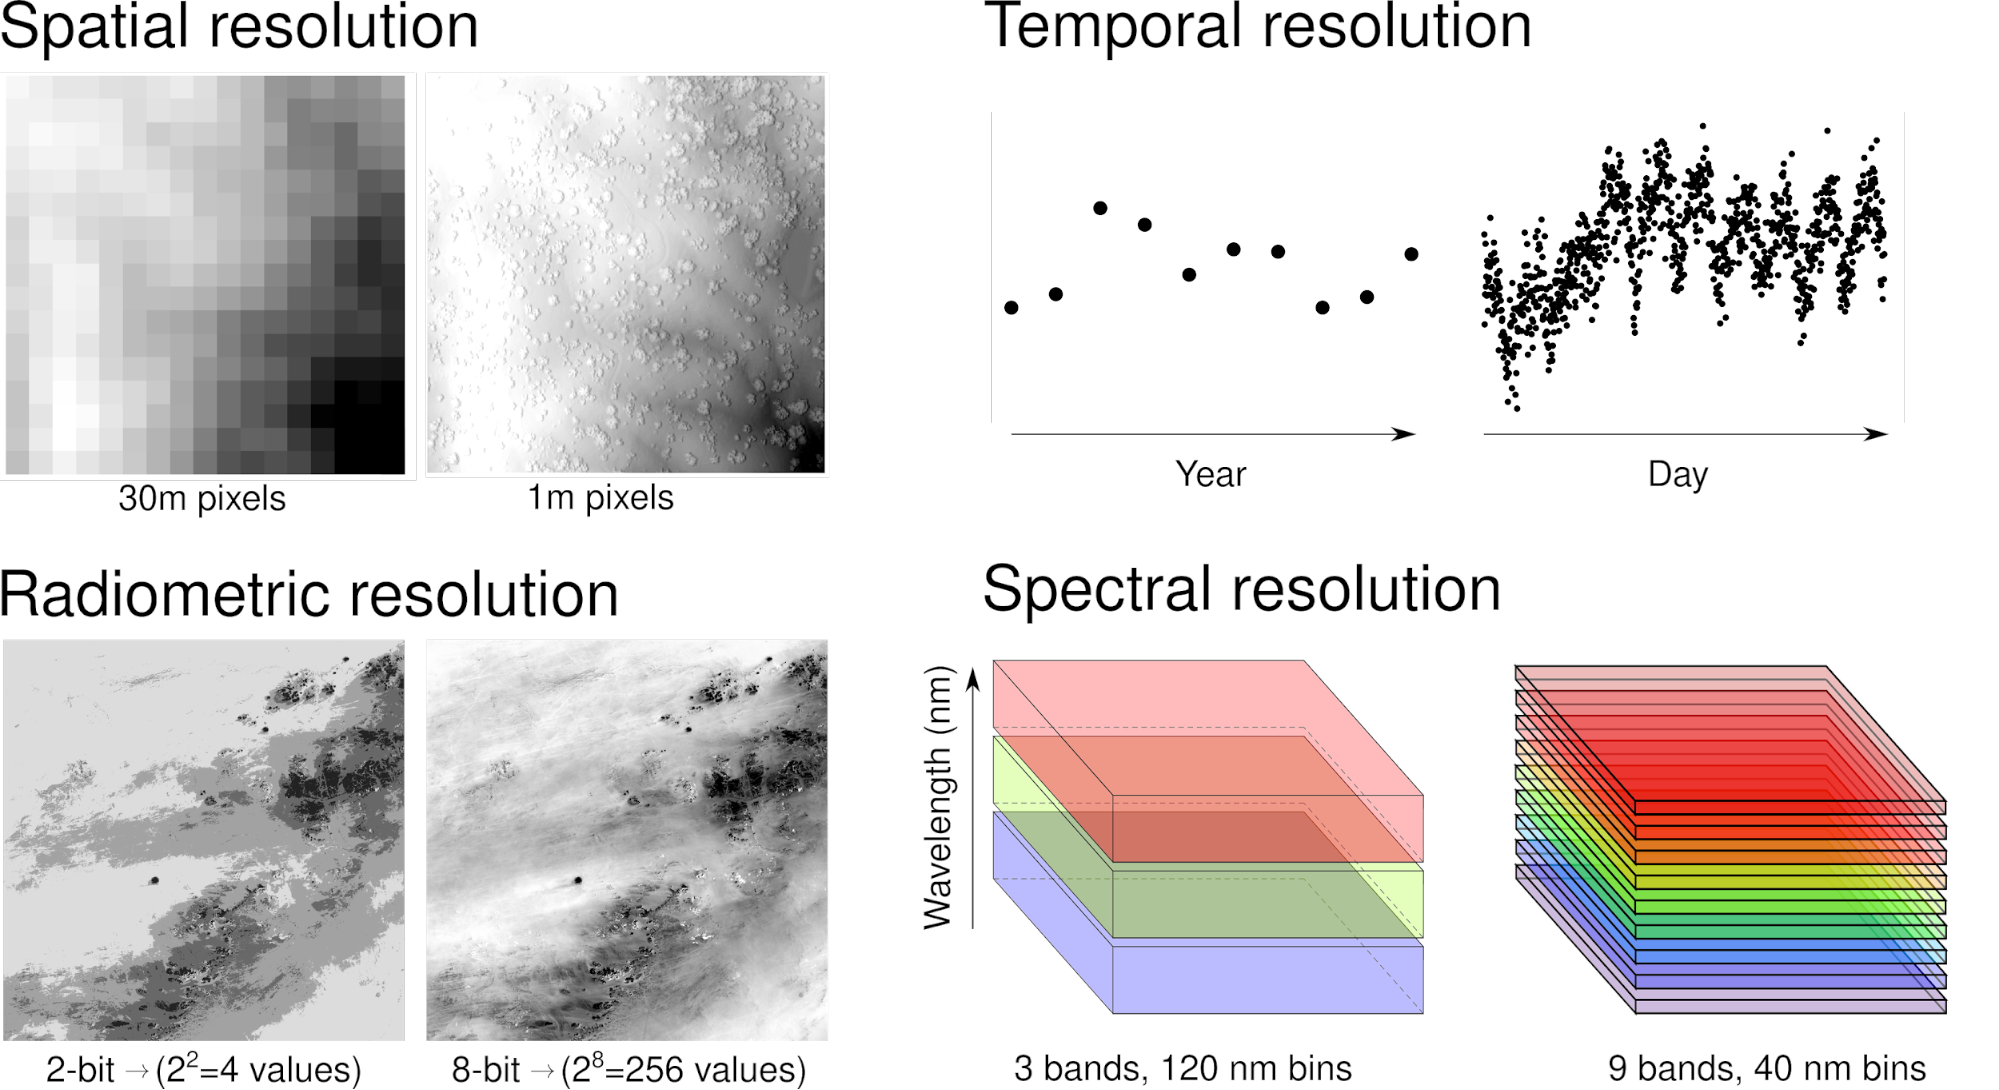
\includegraphics{Figure1.png}
\caption{Different kinds of resolution, with examples of lower and
higher resolution data. Spatial resolution relates to pixel size,
temporal resolution to observation frequency, radiometric resolution to
the number of unique values, and spectral resolution to binwidth in the
electromagnetic spectrum.}
\end{figure}

\begin{figure}
\centering
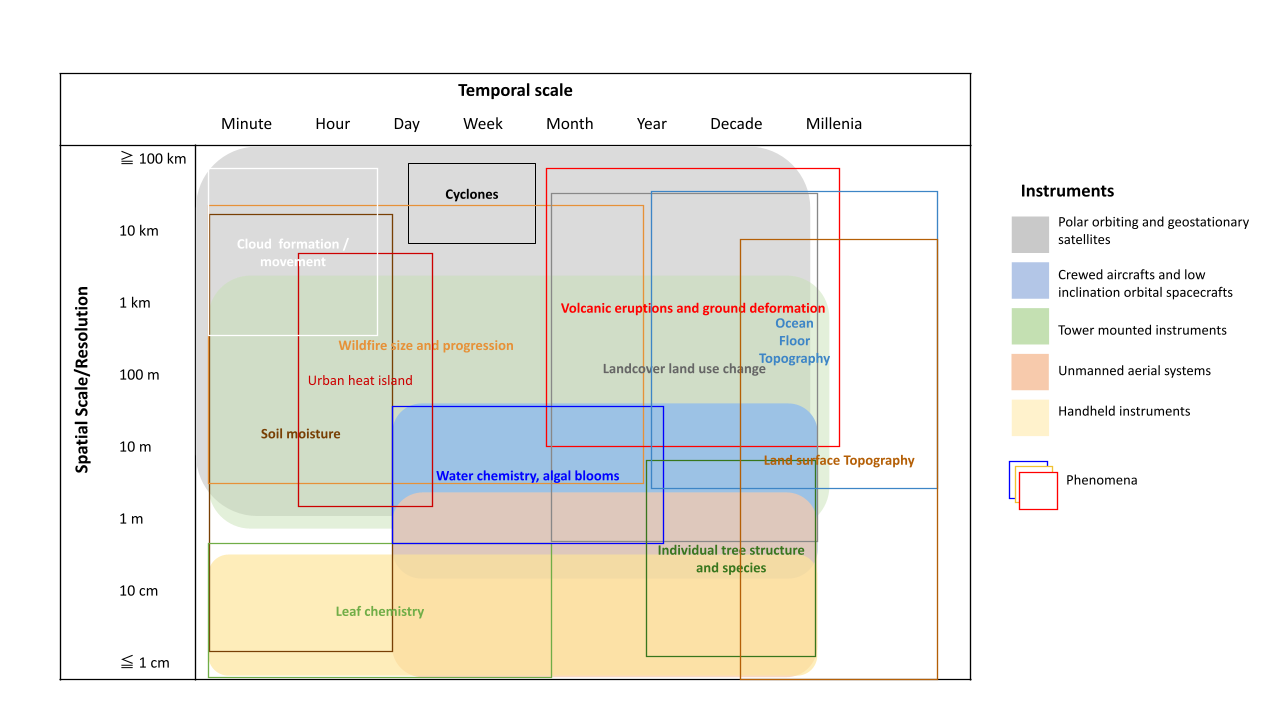
\includegraphics{scale_figure_tsr.png}
\caption{Variations in spatial and temporal scale in phenomena and
remote sensing instruments.}
\end{figure}

\hypertarget{tables}{%
\section{Tables}\label{tables}}

\end{document}
